% -*- pdf: BrettTerespolskyPEIES092014 -*-
%\documentclass{beamer}
\documentclass[ignorenonframetext]{beamer}

\makeatletter
\def\input@path{{./primitives/}}
\makeatother
\usepackage{tikz}
\usetikzlibrary{positioning, arrows, decorations.markings}
\usepackage{pgfplots}
\usepackage{circuitikz}
\usepackage{graphicx}
\usepackage{wrapfig}
\usepackage{verbatim}
\usepackage{url}
\usepackage{siunitx}
\usepackage{graphicx,wrapfig,lipsum}
\pgfplotsset{compat=1.10}
\usepackage{caption}

\tikzset{onslide/.code args={<#1>#2}{%
  \only<#1>{\pgfkeysalso{#2}} % \pgfkeysalso doesn't change the path
}}

\tikzstyle{highlight}=[color=red]

\pgfplotscreateplotcyclelist{linestyles*}{solid,dashed, dotted, loosely dashed, loosely dotted, loosely dashdotted}

	% \pgfdeclaremask{logo-mask}{witseie-logo.mask}
	\pgfdeclareimage[height=1.5cm]{wits-logo}{WITS-logo.jpg}
	%\pgfdeclareimage[height=1.5cm]{iclp-logo}{ICLPlogo.png}
	\pgfdeclaremask{logo-mask}{witseie-logo.jpg}
	\pgfdeclareimage[mask=logo-mask,interpolate=true,height=1.5cm]{witseie-logo}{witseie-logo}
	\logo{\pgfuseimage{wits-logo}}

\mode<presentation>
{
  \setbeamercolor{palette sidebar secondary}{use=sidebar,fg=structure.fg!65!black}

  \useoutertheme[left,height=0pt]{sidebar}
  \usecolortheme{sidebartab}
  \setbeamertemplate{sidebar canvas left}[vertical shading][top=blue!75!black,middle=blue!10!white,bottom=white]
  \setbeamercovered{dynamic}
  \beamertemplatenavigationsymbolsempty

%  \useoutertheme[hideallsubsections,right]{sidebar}
%  \useoutertheme[right]{sidebar}
%  \setbeamertemplate{sidebar canvas right}[vertical shading][bottom=blue!75!black,top=white]
}

\makeatletter
\setbeamertemplate{sidebar \beamer@sidebarside}
{
\beamer@tempdim=\beamer@sidebarwidth%
\advance\beamer@tempdim by -6pt%
{\usebeamerfont{title in sidebar}%
  \vskip1.5em%
  \hskip3pt%
  \usebeamercolor[fg]{title in sidebar}%
  \insertshorttitle[width=\beamer@tempdim,center,respectlinebreaks]\par%
  \vskip1.25em%
}%
\insertverticalnavigation{\beamer@sidebarwidth}%
\vfill
\ifx\beamer@sidebarside\beamer@lefttext%
\else%
  \usebeamercolor{normal text}%
  \llap{\usebeamertemplate***{navigation symbols}\hskip0.1cm}%
  \vskip2pt%
\fi%
\hskip3pt
\insertlogo
% \includegraphics[width=\beamer@tempdim,keepaspectratio]{wits-logo}~%
\vskip2pt
}
\makeatother

\usefonttheme{structurebold}

\title[\color{white}Contents]{Extendible Multi-Dimensional Sparse Array Representations For Data Warehousing}
\subtitle{}
\titlegraphic{\pgfuseimage{witseie-logo} }

\author[]{Catherine Honegger}

\institute{School of Electrical and Information Engineering\\University of the Witwatersrand, Johannesburg, South Africa}%\\Email: my@email.com}

\date{5 October 2017}

\setbeamerfont{subsection in sidebar}{size=\fontsize{4.7pt}{6pt}}
\setbeamercolor*{section in sidebar shaded}{parent=palette sidebar secondary,fg=black}
\setbeamercolor*{section in sidebar}
  {parent=section in sidebar shaded,use={sidebar,section in sidebar shaded},%
   fg=black,bg=white!70!black}

\begin{document}

\frame{\titlepage}

	\begin{frame}
	 	\frametitle[]{Outline}
	 	\tableofcontents
	\end{frame}
	
	\section{Objective}
	\begin{frame}
		\frametitle[]{Objective}
		The aim of the proposed study is to improve the modelling and representation of extendible multi-dimensional sparse arrays so that useful compression and storage techniques can be determined.	
	\end{frame}

	\section{Background}
	\begin{frame}
		\frametitle{Background}
		
	\end{frame}
	
	\begin{frame}
	\frametitle{Big Data Representations}	
	
	\end{frame}

	\begin{frame}
		\frametitle{Sparse Array Representation}	
		
	\end{frame}
	
	\begin{frame}
		\frametitle{Multi-dimensional Array Representation}
			
		
	\end{frame}
	
	\section{Methodology}
	\begin{frame}
		\frametitle{Methodology}
			\begin{figure}
			\centering
			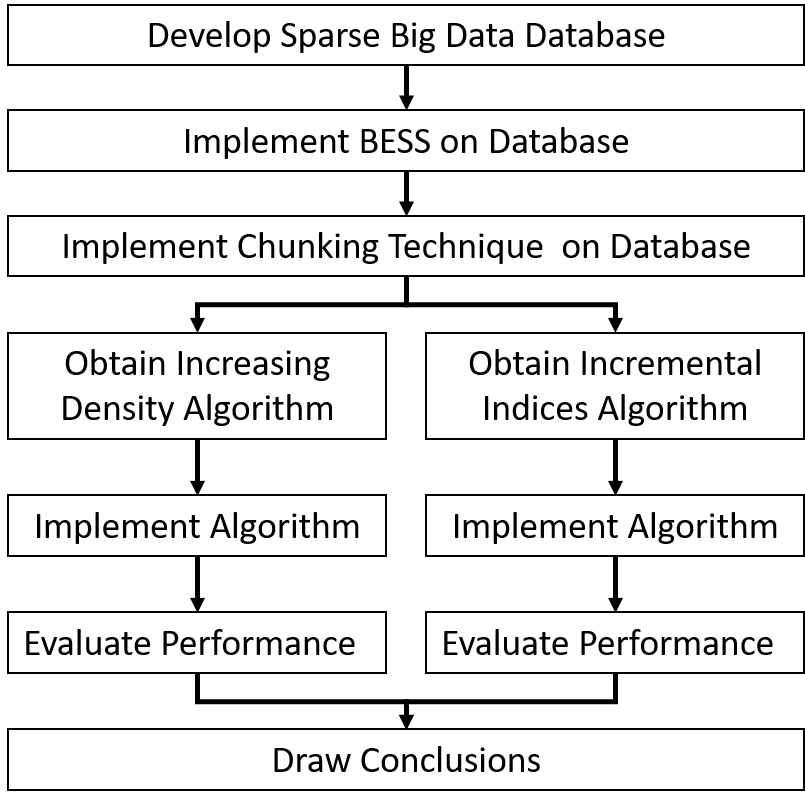
\includegraphics[width=0.51\linewidth]{proposedMethod.png}
			%\caption{System overview}
			\label{fig:system_flowchart}
		\end{figure}
	\end{frame}


	\section{Experimental Set up}
	\begin{frame}
		\frametitle{Experimental Set up}
		\begin{itemize}
			\item Laptop with an Intel(R) Core(TM) i5-2450 multi-core processor at 2.50~GHz and 4GB
			\item Ubuntu 64-bit Linux 16.04.3 LTS.
			\item C using GNU Compiler Collection (GCC) 7.2.
		\end{itemize}
	\end{frame}
	
	\section{Preliminary Results}
	\begin{frame}
		\frametitle{Preliminary Results}
		
	\end{frame}

	\section{Schedule}
	\begin{frame}
		\frametitle{Schedule}		

	\end{frame}
	
	\section{Summary}
	\begin{frame}
		\frametitle{Summary}
		%\begin{itemize}
			
		%\end{itemize}	
	\end{frame}
	
	%\section[]{References}
	\begin{frame}
		\frametitle{References}
		\fontsize{7.5pt}{3.9pt}
%		\begin{itemize}
%			\item T. Economist. "The World's Most Valuable Resource." The Economist, vol. 423, no. 9039, p. 7, May 2017.
%			\item M. Golfarelli and S. Rizzi. Data Warehouse Design: Modern Principles and Methodologies, chap. 1, pp. 1{42. India: McGraw-Hill Professional, first ed., Jan. 2009.
%			\item H. Wang. Sparse Array Representations And Some Selected Array Operations On GPUs. MSc Dissertation, University of the Witwatersrand, Johannesburg, South Africa, Jul. 2014.
%			\item E. J. Otoo and D. Rotem. "Efficient Storage Allocation of Large-Scale Extendible Multi-dimensional Scientific Datasets." In 18th International Conference on Scientific and Statistical	Database Management, pp. 179{183. IEEE, 2006.
%			\item B. Twala. "Big Data for Africa." presentation, Feb. 2017.
%			\item N. E. Moukhi, I. E. Azami, and A. Mouloudi. "Data Warehouse State of the art and future challenges." In 2015 International Conference on Cloud Technologies and Applications (CloudTech). Marrakech, Morocco: IEEE, Jun. 2015. URL http://ieeexplore.ieee.org/abstract/document/7337004/.
%			\item G. Nimako, E. J. Otoo, and D. Ohene-Kwoe. "Chunked Extendible Dense Arrays for Scientific Data Storage." In 41st International Conference on Parallel Processing Workshops, pp. 38{47. 2012. URL http://ieeexplore.ieee.org/document/6337461/.
%			\item P. Pedereira. "Cubrick: A Scalable Distributed MOLAP Database for Fast Analytics." In VLDB 2015 PhD Workshop. Very Large Data Base Endowment Inc., Hawaii: Springer-Verlag, Jul. 2015. URL http://www.vldb.org/2015/wp-content/uploads/2015/07/pedreira.pdf.
%			\item E. J. Otoo, H. Wang, and G. Nimako. "Multidimensional Sparse Array Storage for Data Analytics." In IEEE 18th International Conference on High Performance Computing and Communications; IEEE 14th International Conference on Smart City; IEEE 2nd International Conference on Data Science and Systems, pp. 1520{1529. 2016.
%			\item S. Goil and A. Choudhary. "BESS: A Sparse Storage Structure of Multi-dimensional Data for OLAP and Data Mining." Tech. Rep. CPDC-TR-9801-005, Centre for Parallel and Distributed Computing, Northwestern University, 1997.
%			\item H. W. E.J. Otoo, G. Nimako. "New Approaches to Storing and Manipulating Multi-Dimensional Sparse Arrays." In SSDBM 2014 , 41. ACM, 2014. URL http://dl.acm.org/citation.cfm?id=2618281.
%			\item G. Nimako. Chunked Extendible Arrays and its Integration with the Global Array Toolkit for Parallel Image Processing. PhD Dissertation, University of the Witwatersrand, Johannesburg, South Africa, Oct. 2016.
%			\item M. I. Foundation. "Strength in Numbers: Africa's Data Revolution." online, 2015.
%			\bibitem{14}C. H. Roth and L. John. United States of America: Cengage Learning, third ed., 2016.
%		\end{itemize}	
	\end{frame}
	
	\begin{frame}
		\huge \centering{Thank you } 
		\begin{center}
			\pgfuseimage{witseie-logo}
		\end{center}		
	\end{frame}
	
\end{document}
